\chapter{Extending Local Feature Based Models of SV Detection in a Discriminative Machine Learning Framework}\label{chap_crf}

In my formulation of a general approach for SV prediction in the MapReduce framework, a crucial phase is the computation of a set of features for each genomic location. In my current implementation of Cloudbreak, these features are the parameters which are estimated by fitting a GMM to the distribution of insert sizes that span that location. However, the nature of these features are purposefully not specified in the algorithmic framework to allow flexibility in the implementation of the framework.

Given a set of arbitrary features that encode information about a set of loci that are connected in a sequence, a natural approach is to apply techniques from machine learning to identify regions of interest in that sequence, rather than the heuristics and noise reduction techniques from signal processing that are used in the Cloudbreak implementation described in Chapter \ref{chap_cloudbreak_impl}. Discriminative machine learning techniques have been applied to SV detection in the packages forestSV~\cite{Michaelson:2012fj} and SVM$^2$~\cite{Chiara:2012ey}. However, neither of these tools use machine learning techniques that take into account the sequential nature of the data. 

\section{SV Detection as a Sequence Labeling Problem}

In the the algorithmic framework for solving the structural variation detection problem in MapReduce that we presented in Chapter \ref{chap_framework}, we reduced the problem to one of computing a set of features that described the short read evidence for SVs at each of a set of small regions along the genome. These are then transformed into variant calls by a function which examines the features along each chromosome of the reference sequentially and identifies contiguous blocks of regions with features values that combine to coherently indicate the presence of a variant. This latter part of the process, which we named the \textsc{Postprocess} function in Algorithm \ref{cb_algo}, can be thought of as a sequencing labeling problem based on sequence features. To take the example of deletion detection, we could define two labels: ``Deletion'' if the window participates in a deletion variant, and ``No Deletion'' if it does not. More formally, we can let $Y_i$ be the label at genomic window $i$, where $1 \le i \le n$ where $n$ is the number of windows in the chromosome. If we similarly name the features for genomic window $i$ $X_i$, we can then refer to the entire sequence of labels and features as $Y$ and $X$, respectively.

The goal of fhe \textsc{Postprocess} function, can be broken down into two parts: first, to assign a label to each window in the reference sequence, and second, to consolidate neighboring windows with the same label into variant calls which affect larger regions. Using this model to think about the implementation of Cloudbreak described in Chapter \ref{chap_cloudbreak_impl}, we used a simple linear threshold on the likelihood ratio of the insert size data to label each window, and then consolidated neighboring windows with hand-tuned rules such as the median filter and restriction on the estimated mean of the second GMM component. These latter rules were made necessary by the noisy nature of the data and the simplicity of the window-labeling procedure. However, if we had a completely accurate window-labeling procedure, we could remove much of the complexity of the consolidation step. Since real world data is noisy, however, the best that we can do is to try to find the most likely sequence of labels given the observed data:

\[ \argmax_Y P(Y|X) \]

To acheive the goal of a more principled and more accurate window-labeling procedure we would need to be able to take into account information from multiple features, as well as the labels of nearby windows. In other words, the label of each window should be dependent not only on the observed features at that window but also on the labels of other windows nearby. Probabilistic graphical models provide a framework for defining and learning models that describe these types of dependencies. \todo{Describe PGMs here} One class of graphical model that has been used extensively for sequence labeling tasks in bioinformatics are Hidden Markov Models (HMMs). \todo{describe HMMs}

\section{Integrating Features with Conditional Random Fields}

To overcome these drawbacks of HMMs, we implemented a linear-chain conditional random field~\cite{Lafferty:2001:CRF:645530.655813} model to label genomic deletions. The model was developed using Factorie~\cite{mccallum09:factorie}. Factorie is a toolkit written in Scala that supports a wide variety of factor-graph based models, trainers, and tools, particularly for NLP tasks such as named entity recognition. Our Factorie-based implementation of a structural variation detection program consists of two parts: a modular and configurable set of code for data management of features defined along the genome, along with conversion of real-valued features into into binary binned feature values, and code to construct, train, and run inference on linear-chain CRF models. The code developed for this project was written in Scala and is available on GitHub at \url{http://github.com/cwhelan/svfactorie}. 

\todo{Feature management. Integration of disparate tracks. Selection of windows. Cumulative vs discrete binning.}

\todo{Model training}

We developed a linear chain CRF model in Factorie. For optimization during training we use the LGBFS algorithm with L2 regularization. We have also experimented with other optimizers including the online AdaGrad regularized dual averaging algorithm \cite{Duchi:2011:ASM:1953048.2021068} with L1 regularization but did not see large differences in preliminary testing. To conduct inference we use the Viterbi max-product belief propogation algorithm.

\section{Features for SV Detection}

As described in Chapter \ref{chap_background}, there are three main signals available for SV detection in short read sequencing data sets: those that come from read pairing information, those that come from read depth, and those that come from split reads. The creation of a discriminative machine learning framework as described above can be used with any arbitrary set of features. Therefore it is possible to create feature sets that combine information from all three SV detection signals and integrate them into this framework. In addition, we can model interactions between features and use those in our predictions. Finally, the arbitrary nature of the feature function allows us to incorporate prior knowledge about given genomic regions, including sequence annotations. We have constructed a feature set that includes all of these types of features, as described below:

\subsection{Read Pair Features}

Read pair features are those that are based upon the inferred insert sizes and orientations linking paired reads, as described previously. We use the following RP features:

\begin{itemize}

\item The three features generated by Cloudbreak and described in Chapter~\ref{chap_cloudbreak_impl}: the log likelihood ratio of the insert sizes observed at each window in the two-component GMM fit vs. the likelihood under the expected normal distribution for the sample; the estimated mean $\mu_2$ of the second component of the two-component GMM, and $\alpha$, the estimated weight of the second component in the two-component GMM.

\item Insert size change point features: in addition to the insert size calculations described in the Cloudbreak implementation, we also wanted to consider alternative features based on insert sizes. In particular, we wanted to test whether the addition of features that indicate whether a window represents a point at which the insert size distribution in a local surrounding region is changing would improve identification of variants. We compute such a score as follows: let $i$ be the index of a window in the genome, and $S_{i..j}$ be the list of observed insert sizes spanning the windows labeled $i$ through $j$. Now consider a local neighborhood of size $n$ which comprises the windows $i-\frac{n}{2},...,i,...,i+\frac{n}{2}$. Let $\Theta_{i..j}$ be model parameters that can be estimated from the distribution of insert sizes $S_{i..j}$, and $P(S_{i..j}|\Theta_{i..j})$ be the likelihood of observing $S_{i..j}$ under the model with parameters $\Theta$. We can calculate a change score for each window $i$ by examining the likelihood of the data in the halves of the neighborhood to the right and left of that window, by estimating $P(S_{i-\frac{n}{2}..i})$ and $P(S_{i+1..i+\frac{n}{2}})$. Simultaenously, we can perform the same estimates for all of the data in the neighborhood and compute $P(S_{i-\frac{n}{2}..i+\frac{n}{2}})$. The likelihood ratio between these two models:

\[ \frac{P(S_{i-\frac{n}{2}..i}) * P(S_{i+1..i+\frac{n}{2}})}{ P(S_{i-\frac{n}{2}..i+\frac{n}{2}})} \]

then serves a score indicating the presence of a change between the segments to the left and right of point $i$. This has the advantage of being a parameter-free calculation, since parameters are re-estimated from each segment for each calculation. According to the Cloudbreak's model, it would be natural to estimate two component GMMs for each segment of insert size data. However, in practice we found that changes were well captured by the likelihood ratio score when only a single-component Gaussian is used for each segment, and so we have used that model for the sake of efficiency. We use a neighborhood size of 200 bp.

\end{itemize}

\subsection{Split-read features}

Split read signals are caused when a read overlaps a genome breakpoint, disrupting the full alignment of that read. If only simple variants are considered, such a scenario should reveal the exact location of the breakpoint. However, these are difficult to resolve in practice, because the algorithm must first identify potentially split reads from those that fail to align or partially align, and then align the two ends of the split read to the genome, potentially at large distances from one another. True split-read based SV detection methods use dynamic programming and heuristics to try to accomplish this; however, the difficulty of doing so with current read lengths means that they have low sensitivity (although very high specificity). Rather than conduct an exhaustive split read alignment search, we instead use indirect evidence of split reads that can be extracted from standard first-pass alignments:

\begin{itemize}
\item Soft clipping: When reads are aligned to the genome by short read mappers like BWA, they can in some cases be only partially aligned. In BWA, this occurs when a parameterized clipping penalty is less than the additional cost of aligning the rest of the read according to a Smith-Waterman dynamic programming alignment. Aligners refer to this "soft clipping", and flag the read with specific indicators when it occurs. Although there are other possible reasons for soft clipping (for example, the quality could fall at the end of the read, producing many erroneous mismatches wit the reference), this could potentially be indicative of a structural variation breakpoint disrupting the read's alignment to the reference. For integration into the CRF feature set, we created a feature track that counts the number of times a soft clip occurred in each 25bp genomic window.

\item Singleton alignments: For paired end reads, sometimes only one read in the pair can be successfully aligned to the genome. These are referred to as "singleton" alignments. Potentially a singleton alignment could indicate that the other read in the pair contains a variant that prevented it from being aligned, and therefore that a breakpoint could lie somewhere within the distance of the insert size, or could have disrupted the alignment of the other read in the pair. We count the number of singleton alignments in each window. \todo{Visually inspecting the data, and looking at the trained weights in my model, this doesn't seem like a very useful feature in practice.}
\end{itemize}

\subsection{Read depth features}

The third major signals of structural variations from short-read sequencing data are related to read depth. In the context of deletions, one would expect to see fewer reads aligning to sections of the genome which have been deleted in the sample; if the deletion is 100\% represented in the sample and is homozygous, any reads aligning to that location must be incorrect alignments. In practice, coverage depth is affected by lots of noise resulting from incorrect mappings and biases of the sequencing process (for example, the amount of GC content in a given fragment of DNA will affect its representation in the sequencing data set). 

\begin{itemize}
\item Coverage depth: As one feature, we calculate the average coverage depth of each base in each 25bp window.

\item Coverage change points: We applied the change point detection algorithm outlined in the previous section to identify windows at which the coverage changes. Although we experimented with different neighborhood sizes, we found that this was not a very valuable feature for breakpoint identification. For the results reported below, we used a neighborhood size of 600bp.

\item Coverage Drops: We speculated that for the specific case of deletion detection, the most informative coverage statistic might be one that indicates whether or not the coverage at a given window drops relative to its local neighborhood. Therefore, we compute for each window the drop in coverage depth from the mean coverage depth of the windows that lie in the surrounding 500bp.
\end{itemize}

\subsection{Genome annotations}

Finally, the ability to include arbitrary features in the model allows us to incorporate prior knowledge about the genome into our feature set. In particular, some types of genomic features frequently cause incorrect alignments; training the model based on those feature annotations could help the variant caller calibrate its confidence in each prediction.

\begin{itemize}
\item Repetitive regions: We took the UCSC RepeatMasker track for the reference genomes used in the testing and training sets and created a binary feature for each window in the genome, which was true if the window overlaps with a repetitive element designated by RepeatMasker \cite{repeatmasker}.

\item Simple repeats: these are a subset of the repetitive regions track that are made up of repeated k-mers of lengths from one to six. Simple repeats are very difficult to align to, and are therefore the source of many alignment errors. We set a binary feature for each window if it overlapped with an element from the UCSC Simple Repeats track \cite{Benson01011999} for the reference genome.

\item Segmental duplications: These are larger regions (10kb+) that have at least one other copy in the genome with high sequence similarity between the two regions, and are again the source of many alignment errors. We used the UCSC Segmental Duplications track to set binary features on each window in the genome.

\end{itemize}

\subsection{Binarization of real-valued features}

Although conditional random fields can support real-valued features, the fact that they are linear models means that it is often helpful to convert real-valued features into related set of binary-valued features for labelling problems. For example, this can help prevent the domination of the output by single real-valued features with very high values. Therefore, we built two binarization schemes into our codebase for real valued features. The first allows the user who is training the system to specify a set of cut points $c_{1..k}$ which divide the range of the variable into $k + 1$ bins. If the value of the feature lies in bin $i$, the system sets binary feature $b_i$ to true and all others to false. The second binarization procedure is a cumulative binning scheme. Again, the user specifies cut points which divide the range of the variable into $i$ bins. In this case, however, binary features are set to true for bin whose end point is greater than or equal to the actual value of the variable. To specify all feature definitions and their types, the user defines each feature variable, its location in the training and test data files, the binning scheme, and the cutoff points for binning. Table~\ref{crf_feature_definitions} shows the feature definitions used for the results reported later in this chapter. This scheme allows for rapid testing of different feature combinations and binning schemes, depending on what data is available.

\begin{table}
\begin{center}
\footnotesize
\begin{tabular}{rrrp{3.5cm}r}
 \hline
Feature Name & Type & Column & Description & Cutpoints \\
 \hline
 mu1 & binnedReal & 1 & $\mu_2$ from Cloudbreak GMM  &  260.0,340.0 \\
 lr &  cumulativeBinnedReal  &  2   & Likelihood Ratio from Cloudbreak GMM &  0.75,2.5,10.0,75.0,500.0 \\
 singletons & cumulativeBinnedReal &  6  & Singleton alignments  &  1.0,2.0 \\
 changePoint & cumulativeBinnedReal & 7 & Insert size change point & 5.0,15.0,50.0 \\
 softClip & cumulativeBinnedReal & 8 & Soft clipped alignments &  1.0,2.0,3.0 \\
 rdepth & cumulativeBinnedReal & 9 & Average read depth & 0.1,0.25,0.5,0.75,1.0 \\
 covChangePoint & cumulativeBinnedReal &  10 & Depth of coverage change point scores &  10.0,20.0,30.0 \\
 covDrop20 &  cumulativeBinnedReal  &  11 & Coverage drop &  5.0,10.0,20.0 \\
 simpleRepeat & boolean &  13  & Simple Repeat & \\
 repeat & boolean &  14  & Repeat & \\
 segdup & boolean &  15  &  Segmental Duplication & \\
 \hline
\end{tabular}
\end{center}
\caption{Feature definition for the CRF training and test data. Each line indicates the feature's name and type, as well as the type of binning scheme (simple or cumulative), and the cut points to use when binning.}
\label{crf_feature_definitions}
\end{table}

\subsection{Interaction and neighbor features}

I've been adding lots of features and hoping that the optimizer / regularizer will help to find the right ones. To that end, in addition to adding the features defined above to each bin, I also add as separate features: interaction terms for all of the features for the current bin, the features of the bins immediately preceding and after the current bin, and the features of the bins within a certain radius of the current bin (currently 7 neighboring bins).

Figure \ref{crf_features_example} shows an example deletion from the NA18507 gold standard data set, along with tracks showing each of the features described above, as well as the original Cloudbreak call identifying the deletion and a call made by running inference on the trained CRF model.

\begin{figure}
\centering
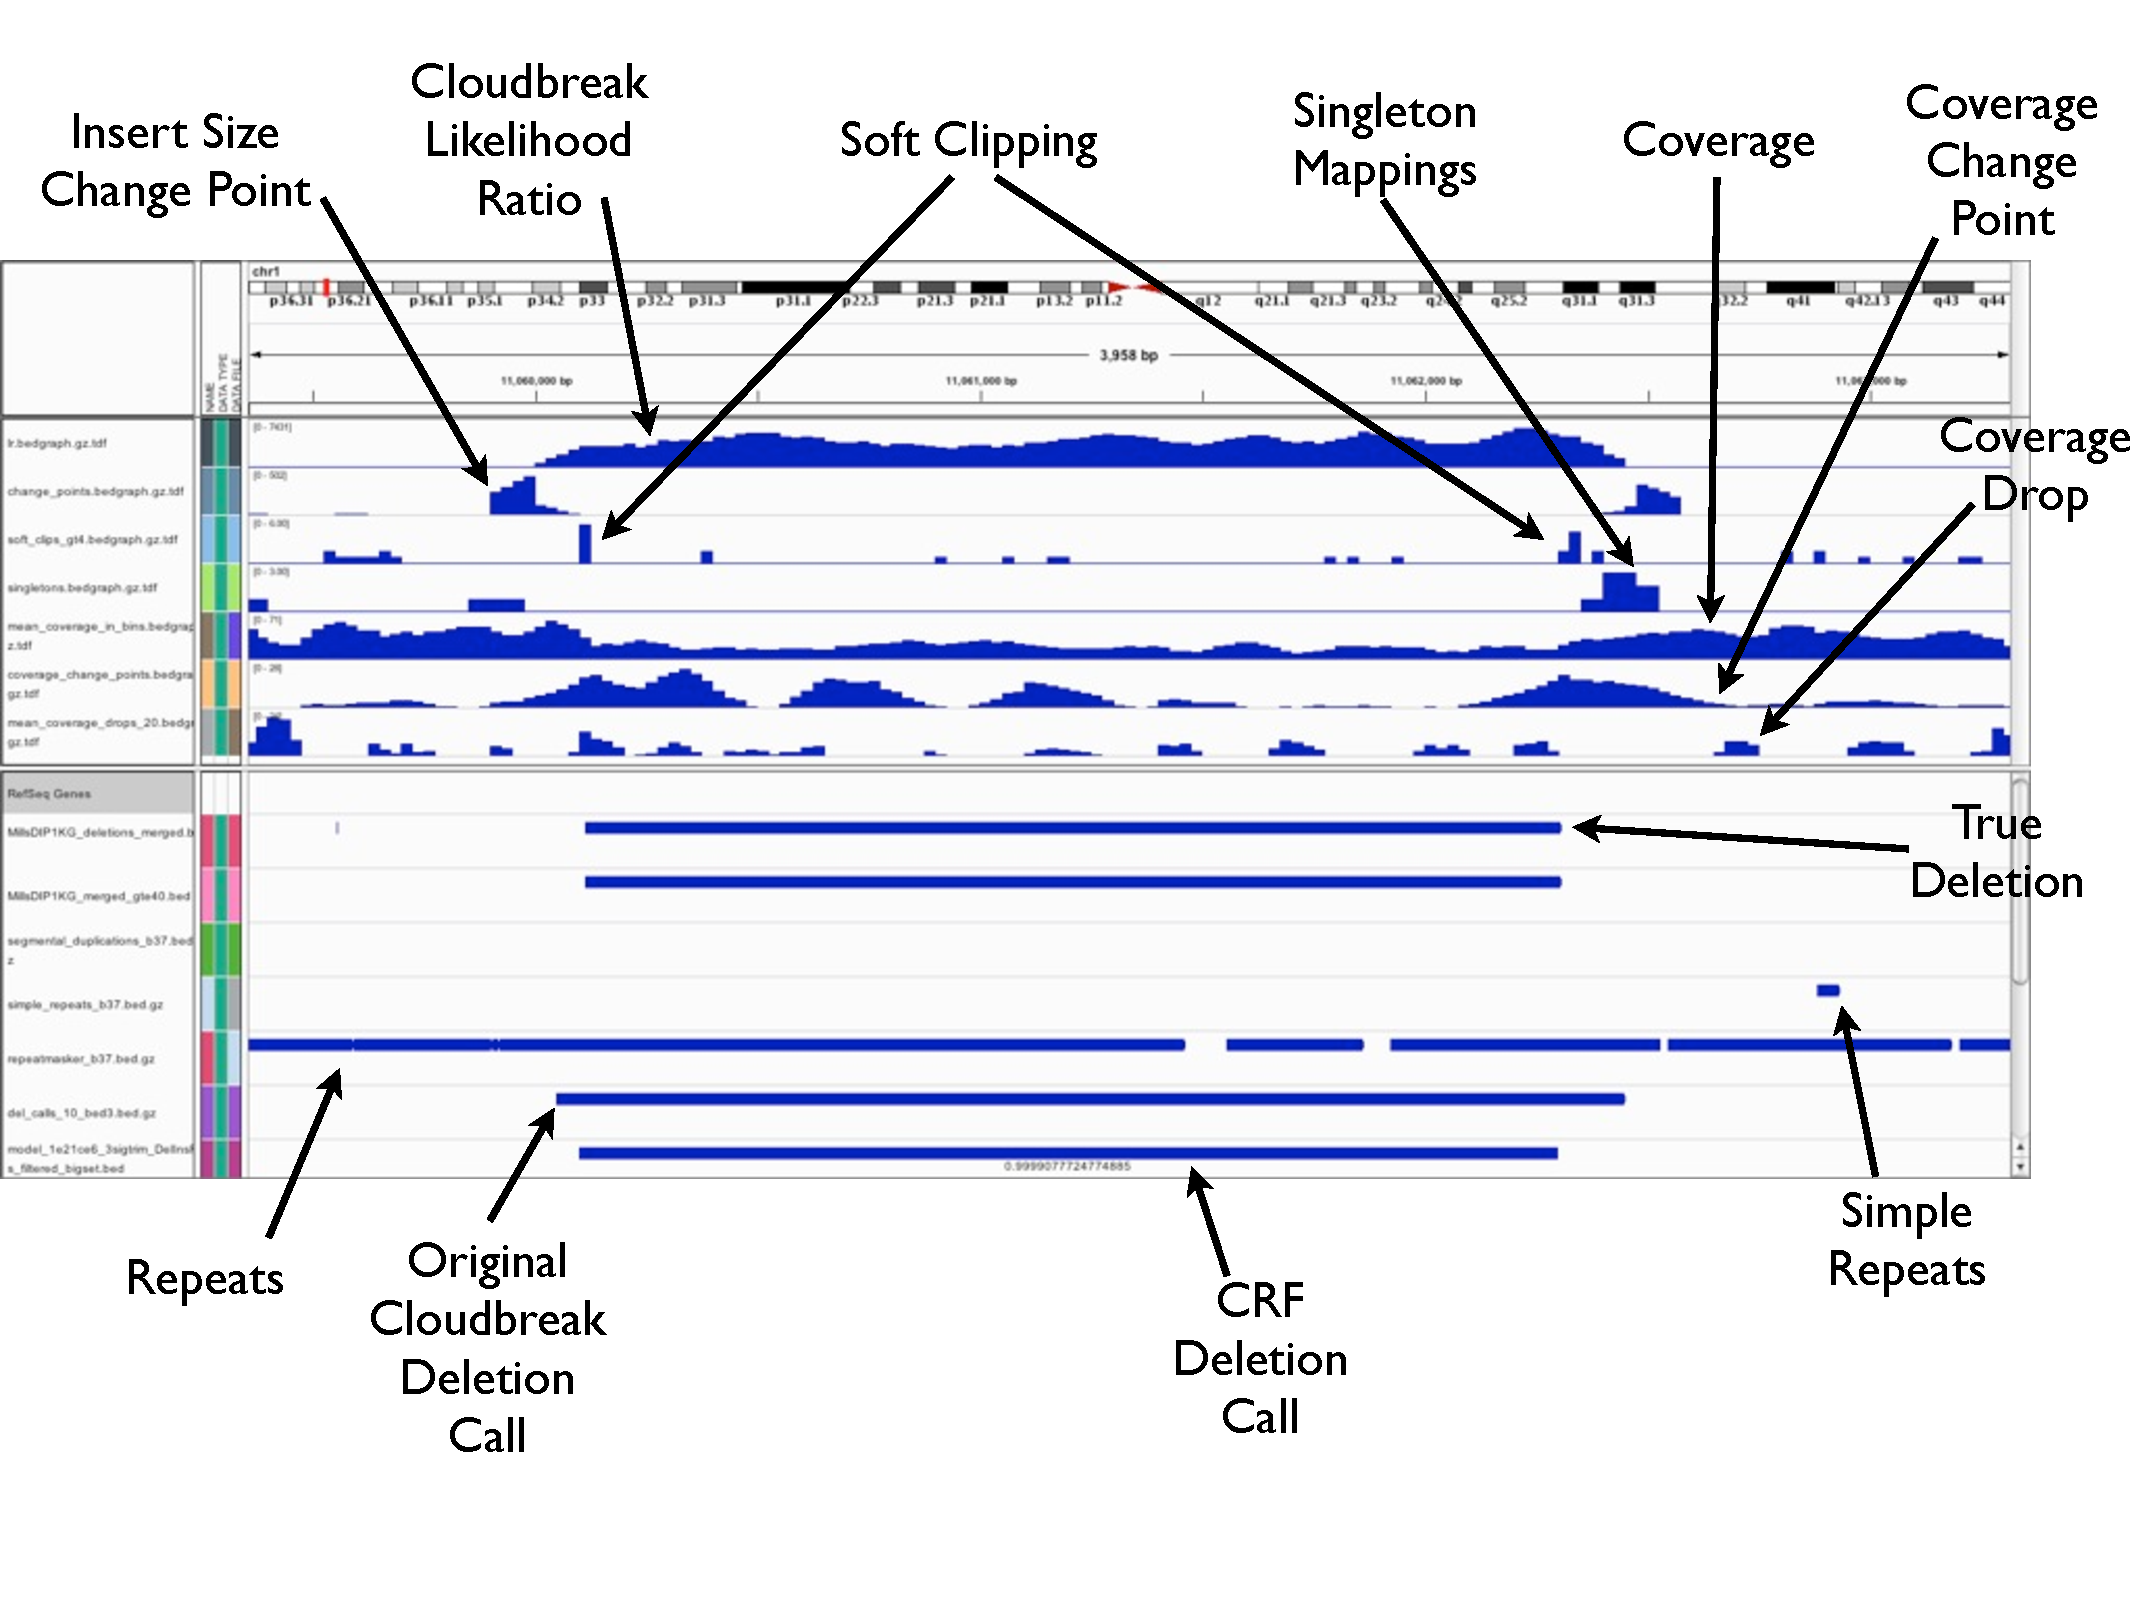
\includegraphics[width=.8\textwidth]{true_example_with_features.pdf}
\caption{An example deletion from the NA18507 data set. The true deletion is shown in track 8. Features shown are in each track are: 1) Likelihood ratio of distribution of insert sizes. 2) Insert size change points. 3) Number of soft clipping events in each window. 4) Number of singleton mappings in each window. 5) Read coverage in each window. 6) Coverage change points. 7) Coverage drops. 11) Simple repeats. 12) Repeats. The original Cloudbreak call is shown in Track 13, and a call made by running inference in the CRF model is shown in Track 14.}
\label{crf_features_example}
\end{figure}

\section{Improving Cloudbreak Calls with CRF Predictions}

\section{Training and Evaluation}
First, I had to decide what data to train and test on. Since we don't have complete annotations of real data sets available, I decided to try training on simulated data. For this, I took my original simulation of chromosome 2 that I did for my Cloudbreak paper and expanded it to a whole genome to try to get more training data, and make the problem a little harder. This simulation includes all of the insertions and deletions annotated for J. Craig Venter's genome. For deletions and insertions with a length over 40bp, there are 5,610 deletions and 6068 insertions. I simulated 30x coverage 100bp paired-end reads with an insert size of 300bp and realigned them to the genome using BWA, as I did for my earlier work. For my test set, I'm using the same data set for individual NA18507, which is 37X coverage with high-quality 100bp paired end reads with an insert size of 300bp. As in my previous work, I then divided both training and test sets into windows of 25bp and computed features for each window.

I also had to choose what data from these sets to feed to the model for training and testing. I ended up creating training windows centered on all of simulated insertion and deletion variants, with flanking regions added on either end. In some runs I've also added all of the Cloudbreak deletion calls made at a very sensitive threshold, so that I could get a lot of false positives into the training set. 

To pick regions to test on, I'm taking the approach of rapidly identifying candidate regions using a fast tool (Cloudbreak in this instance), adding flanking regions to them, and then running the CRF model on those candidate regions to try to label the true variants. This will of course limit the recall of the CRF approach to the recall of the candidate regions I pick but this strategy seemed like a more efficient one than trying to label the entire genome.

\begin{figure}
\centering
\includegraphics[width=\textwidth]{/Users/cwhelan/Documents/svpipeline/figures/NA18507_DELS_ROC_with_CRF.pdf}
\caption{ROC curve showing the accuracy of Cloudbreak calls that have been verified and refined with conditional random field predictions (Cloudbreak-CRF)}
\label{roc_NA18507_with_crf}
\end{figure}

\begin{figure}
\centering
\includegraphics[width=.8\textwidth]{/Users/cwhelan/Documents/svpipeline/figures/breakpointResolutionNA18507_withCRF.pdf}
\caption{Breakpoint resolution of each tool's successful predictions on the NA18507 data set, including Cloudbreak calls which were verified and refined with CRF predictions (Cloudbreak-CRF)}
\label{breakpoint_resolution_NA18507_with_crf}
\end{figure}

\section{Discussion}

As an alternative to CRFs, I will also investigate the use of deep learning techniques such as sequential deep belief networks~\cite{andrew2012:sdbn}, which have been used successfully in sequence processing tasks in speech recognition and other domains.

The outcome of this extension will be: the creation of a training, development, and test set, along with a feature generation scheme and description of the model used; an evaluation of the performance gains that can be achieved, with a comparison to other SV detection approaches; and a discussion of the benefits and drawbacks of using such an approach.
